\documentclass[a4paper, onecolumn, 12pt]{article}
\usepackage[left=33mm,right=33mm,top=35mm,columnsep=15pt]{geometry} 

% basic packages
\usepackage[english]{babel} %language
\usepackage[utf8]{inputenc} %input encoding
\usepackage{float} %position of floating objects
\usepackage{bookmark} %hyperlinks in pdf
\usepackage{subcaption}
\usepackage[T1]{fontenc}
\usepackage{lipsum} %placeholder text

% math packages
\usepackage{amsthm} %theorems
\usepackage{amsmath} %math
\usepackage{mathtools} %still math

% code packages
\usepackage{listings} %code
\usepackage{xcolor} %syntax highlighting
\usepackage{algorithm}
\usepackage{algpseudocode}
\usepackage{fancyvrb}

% todonotes package
\usepackage{xkeyval}
\usepackage{tikz}
\usepackage{calc}
\setlength {\marginparwidth }{2cm}
\usepackage{todonotes} % Load the todonotes package

% custom commands
\newcommand\tab[1][.3cm]{\hspace*{#1}}
\newcommand\tabeq[1][.5cm]{\hspace*{#1}}

% \usepackage{physics}
% \usepackage{adjustbox}
% \usepackage{placeins}
% \usepackage{csquotes}
% \usepackage[normalem]{ulem}
% \useunder{\uline}{\ul}{}

\title{Remote Interaction with a Nao Humanoid in competitive games \\ Elective in AI / HRI Report}
\author{Flavio Maiorana \and Valerio Spagnoli \and Flavio Volpi}
\date{\today}

\begin{document}

\maketitle

\section{Introduction}
\label{sec:intro}

In the context of RoboCup games, robots are fully autonomous and are not allowed
to receive any external help from humans. However, in a world where robots are
used in everyday life, they need to collaborate with humans.
Moreover, the RoboCup 2050 challenge aims to have a football match between the
winning team of the RoboCup and the human winning team of the FIFA World Cup. In
this project, we aim to make a very small step in that direction by developing a
system that allows a human operator to remotely control and interact with a Nao
Humanoid through a graphical interface and a web socket. This pipeline was
specifically designed to be used in the RoboCup 2024 SPL challenge, where two robots
of one team had to compete against two robots of the opponent team, and one of the
two robots for each team was controlled by a human operator. Furthermore, the rules
of the challenge forced the human operator to turn his back to the field, in order
to not directly observe the environment. This constricts us to make use of the 
directional robot-human communication also for the reconstruction of the world model,
useful for the human to decide commands to provide to the controlled robot.


\subsection{Objectives}
\label{sec:obj}

The main objective of the project is to develop a framework that allows the human operator
to use the robot as a proxy to interact with the environment, namely the soccer
field. To do this, a form of bidirectional interaction between the human operator 
and the controlled robot is necessary. The human needs
to be completely aware of the robot's surroundings, that is, the human can
perceive the robot's surroundings only through the robot's sensors. The robot,
on the other hand, has to be able to receive commands from the human operator
and execute them in real-time. The robot should also be able to send feedback to
the human operator in real-time. 
\todo[inline]{Allungare un po' il brodo}
\todo[inline]{Spingerei anche sul fatto che il tutto deve essere utilizzabile in un 
ambiente competitivo}

\section{Solution}
\label{sec:sol}

\subsection{BHuman}
\todo[inline]{Cambiare nome alla sezione}
The framework on which everything stands on is derived from that one of the
German team B-Human \cite{}, University of Bremen. At low level, the robot is 
controlled by three threads:
\begin{itemize}
    \item Cognition: it is responsible for collecting all informations from the 
    environment through cameras and sensors; also, it takes images and informations as input,
    and returns high level commands about the actions the robot has to execute;
    \item Motion: it converts high level commands of the thread Cognition in effective
    motion of the robot;
    \item Debug: it allows a communication between the robot and the host pc for the 
    transmission of debugging information.
\end{itemize}
\todo[inline]{aggiungere immagine dei processi}

The two main components for the collection and storage of information from the environment
are called Representations and Modules.
The former stores the information at the current instant, and they represent the actual overview
of the world. Each representation is a derived class of the class $Streamable$, which allows a 
direct connection of all attributes and functions of our representation with all other
representations and modules.

We opted for a solution that prioritizes high-level commands and audio-visual
feedback. The main component of the system is the graphical interface. It is
made by a bunch of buttons, that allow the human operator to send commands to the
robot, and a 2D representation of the field that shows the robot's position and
its recosntruction of the world.  

\begin{figure}[H]
    \centering
    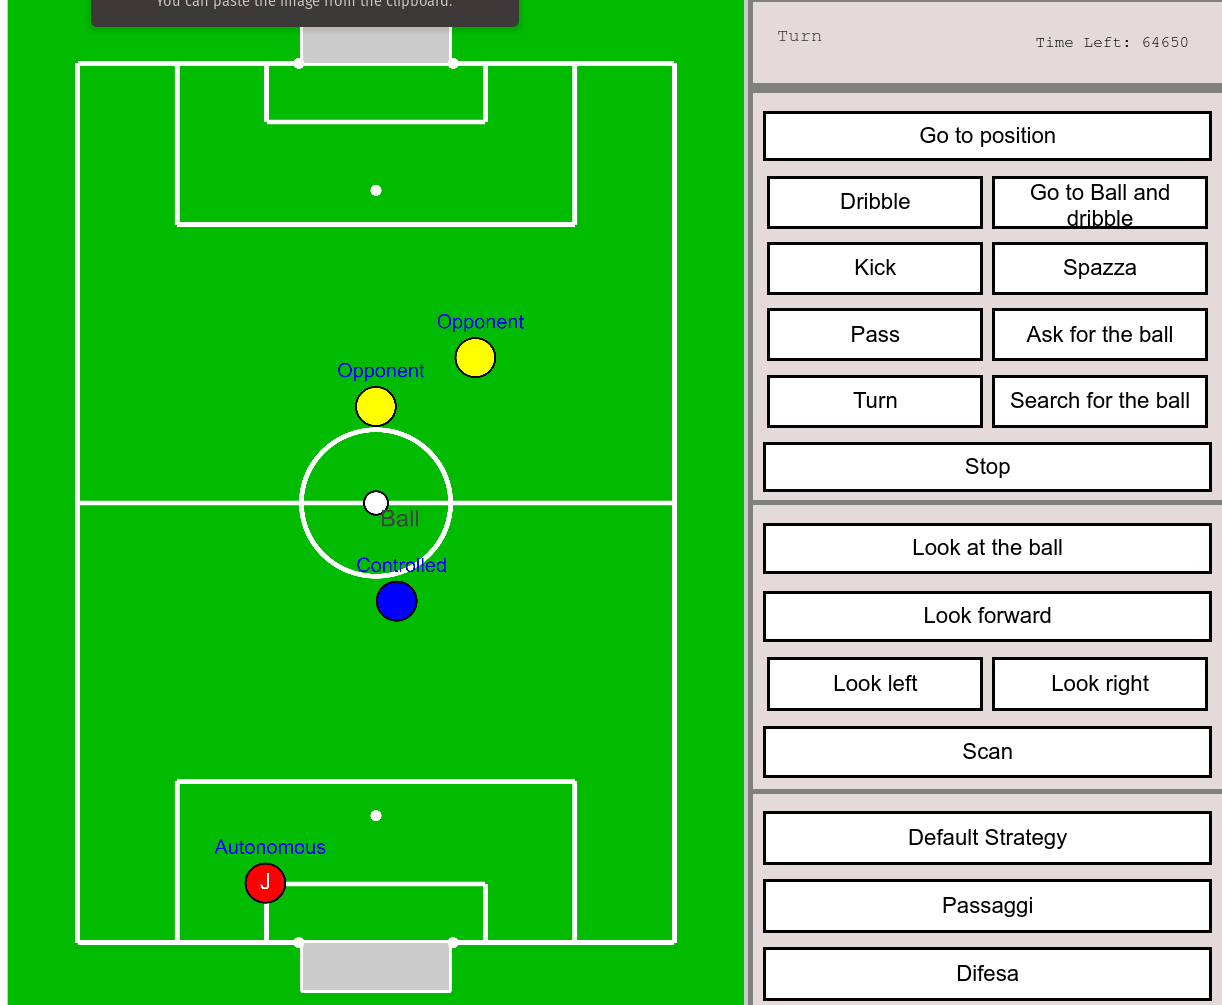
\includegraphics[width=0.9\linewidth]{assets/interface.png}
    \caption{The graphical interface}
    \label{fig:interface}
\end{figure}

\begin{figure}[H]
    \centering
    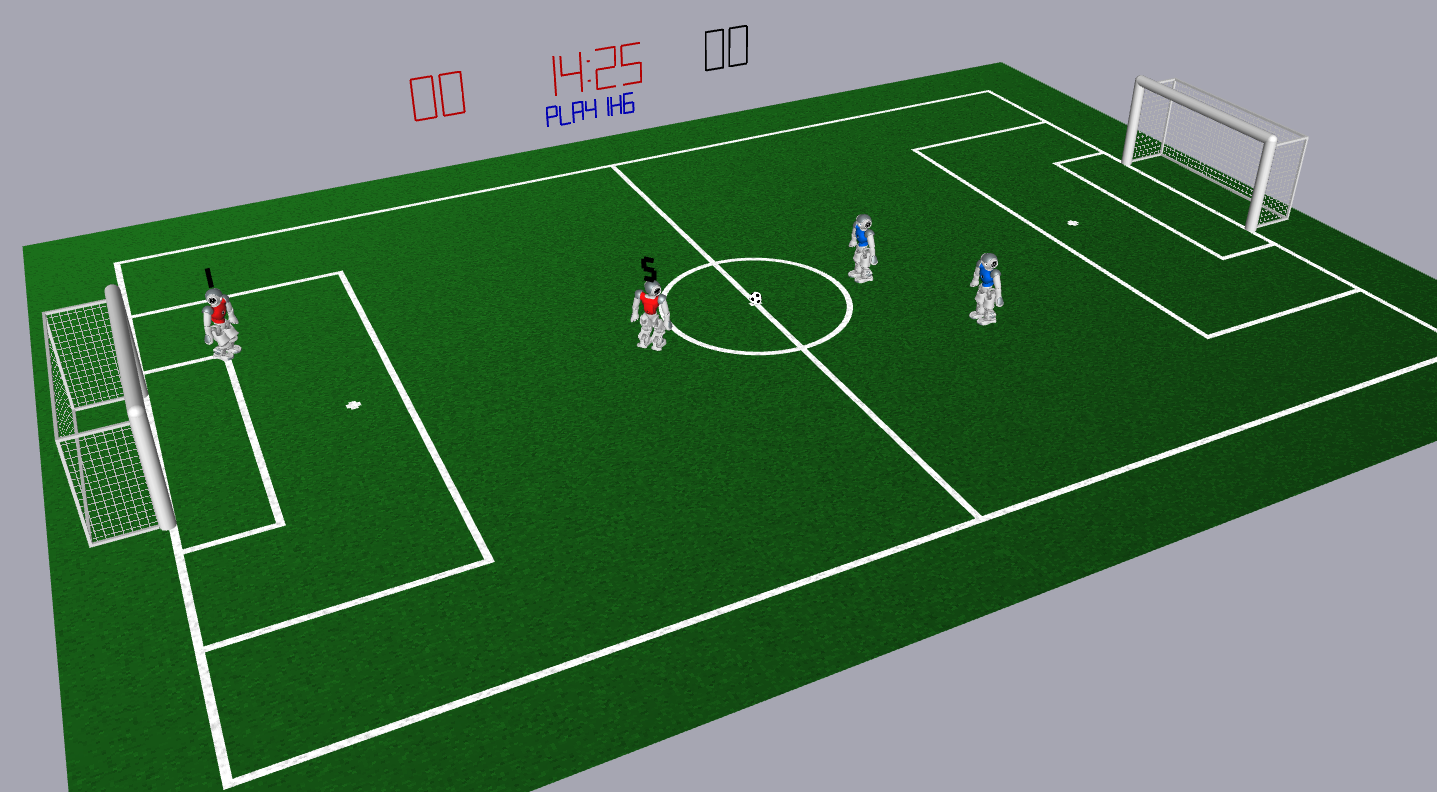
\includegraphics[width=0.9\linewidth]{assets/simrobot.png}
    \caption{The Corresponding Field Configuration}
    \label{fig:nao}
\end{figure}

\section{Implementation}
\label{sec:impl}

\todo[inline]{Dettagli sul codice}

\section{Results}
\label{sec:res}

\todo[inline]{Non so che cavolo metterci qui}

\section{Conclusion}
\label{sec:con}

\todo[inline]{Amen}

\bibliographystyle{unsrt}
\bibliography{references}

\end{document}
